\pdfoutput =0\relax 
\documentclass[
12pt,
a4paper,
twoside,
listof=totoc,		% Abbildungs-/ Tabellenverzeichnis im Inhaltsverzeichnis darstellen
bibliography=totoc,
numbers=noenddot,
draft=true,
BCOR=5mm,
]{scrbook}



%------------------ Packages -----------------------------%
\usepackage{graphicx}					%Bilder einbinden
\usepackage[export]{adjustbox}
\usepackage{amsmath}					%Mathematische Gleichungen
\usepackage[ngerman]{babel}				% deutsche Silbentrennung
\usepackage{caption}					%Bildunterschriften
\usepackage{subcaption}					
\usepackage{longtable}					%für lange Tabellen die über eine Seite gehen
\usepackage{pdflscape}					%Seite drehen
%\usepackage{lscape}
\usepackage[figuresright]{rotating}		%Tabelle in Querformat
\usepackage{pdflscape}
\usepackage{appendix}					%Anhang
\usepackage{booktabs}
\usepackage[utf8]{inputenc}				% wegen deutschen Umlauten
\usepackage{siunitx}
\usepackage{nicefrac}
%\sisetup{locale=DE,tophrase={{ bis }},per=frac,fraction=nice, output-decimal-marker = {,}}
\sisetup{locale=DE, range-phrase={{ bis }}, per-mode = fraction, output-decimal-marker = {,}}
\usepackage[automark,headsepline]{scrlayer-scrpage}	%header und footer einbinden
% fuer Zitate
\usepackage[square]{natbib} 				% necessary for bibliography style natdin
\usepackage{placeins}					%FloatBarrier
\usepackage{float}
\usepackage{ltxtable}
\usepackage{tabu}
\usepackage[hyphens]{url}				% URLs an Bindestrichen umbrechen
\usepackage[breaklinks]{hyperref} 		% Links einfügen (z.B. im Inhaltsverzeichnis)
\usepackage[nohyperlinks]{acronym} 					%Abkürzungsverzeichnis
\renewcommand*{\acsfont}[1]{\normalfont #1}  %% use anything instead of \normalfont. 	
%\usepackage{color}						%einfärben noch unfertiger Texte
\usepackage{pdfpages} %Einbinden von PDF Dateien zum Beispiel weitere bereits fertige PDFs in ein neues PDF einfügen.
\usepackage[draft]{listofsymbols}
\newcounter{savepage}
\usepackage{slashbox}
\usepackage{diagbox}
\usepackage{listofsymbols}
%\usepackage{gensymb}					% ° (grad)
\usepackage{svg}						% Vektorgrafiken
\setlength{\parindent}{0pt}
\usepackage[font={small,it}]{caption}	% Schriftgröße von allen Tabellen- und Abbildungenbeschriftung kleiner machen
\usepackage{scrhack}
\usepackage{bm}							% ändert \boldsymbol
% MATLAB-Codes einbinden
\usepackage{scrhack}
\usepackage{listings}
\lstloadlanguages{Matlab}				% Matlab-Quellcode-Darstellung
%** Einstellungen für "listings" (Quellcode-Darstellung):
\usepackage{xcolor}
% \definecolor{zebg}{rgb}{1,1,.8} %elfenbeinfarbig
\definecolor{darkgreen}{RGB}{69,139,16} %dunkelgrün
\lstset{language=Matlab, commentstyle=\color{darkgreen}, keywordstyle=\color{blue}, stringstyle=\color{red},
	identifierstyle=\ttfamily\color{black}\bfseries, numbers=left, numberstyle=\tiny, breaklines=true, showstringspaces=false,
	%backgroundcolor=\color{zebg},
	numberblanklines=true, frame=single, xleftmargin=0cm, linewidth=1.0\linewidth, basicstyle=\footnotesize, literate=
	{Ö}{{\"O}}1
	{Ä}{{\"A}}1
	{Ü}{{\"U}}1
	{ß}{{\ss}}2
	{ü}{{\"u}}1
	{ä}{{\"a}}1
	{ö}{{\"o}}1
}

\pdfminorversion=7
\DeclareSIUnit{\Million}{\text{Millionen}}
\DeclareSIUnit{\Milliarden}{\text{Milliarden}}
\DeclareSIUnit{\Fahrradkilometer}{\text{Fahrradkilometer}}
\DeclareSIUnit{\km}{\text{km}}
% MATLAB figures einbinden
%\usepackage{subfig}
\usepackage[crop=pdfcrop]{pstool} 		% pstool wird für Ergebnisse von Matlabfrag benötigt
%\usepackage{pgfplots}
\graphicspath{{graph/}}
%
%
%
%\ohead{\headmark}
\automark[section]{chapter}
\setlength{\headheight}{1cm}
\ifoot*{}
\cfoot*{}
\ofoot*[\pagemark]{\pagemark}
%
%
%
%
%
\pagestyle {empty}

\makeatletter 
\def \thepage {\csname @arabic\endcsname \c@page }
\setcounter {page}{23}
\@input {01MasterArbeit.oldaux}
\makeatother 

\begin {document}
\makeatletter 
\immediate \write \@mainaux {\@percentchar <*PSTOOLLABELS>}
\makeatother 

\centering \null \vfill 

\csname @input\endcsname {Bilder/0testFigure.tex}
 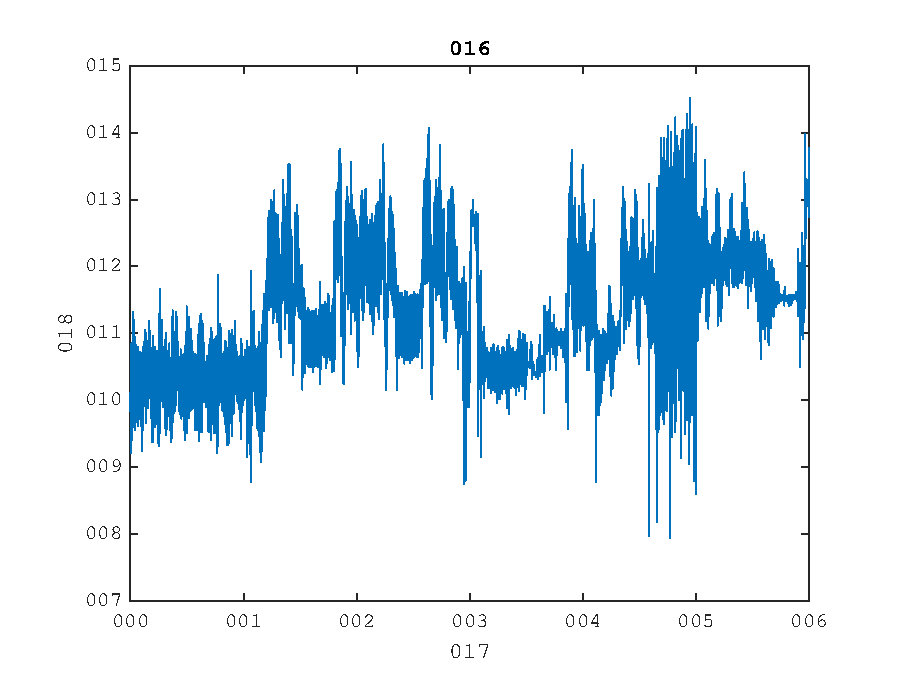
\includegraphics [width=\textwidth ] {0testFigure}

\vfill 

\makeatletter 
\immediate \write \@mainaux {\@percentchar </PSTOOLLABELS>}
\makeatother 

\end {document}

